\documentclass[12pt]{article}
%Gummi|065|=)
\usepackage[a4paper,margin=2.5cm]{geometry}
\usepackage{float}
\usepackage{graphicx}
\title{\textbf{PPRO0605 - Rapport de projet}}
\author{
		BAKALI-HEMOU Yembape\\
		FRANZ Raphaël\\
		MIRGAINE Paul
		}
\date{}

\renewcommand{\contentsname}{Sommaire}

\begin{document}

\maketitle

\section*{Introduction}

Pour la matière PPRO0605, il nous a été demandé de réaliser une application web de gestion des LANs pour la fac. L'application doit être réaliser en PHP et plus précisément, avec le framework Laravel vu en INFO0303. MySql a été utilisé pour la gestion de la base de données. Dans un premier temps, ce rapport se pencheras sur la partie conception de l'application, puis il donneras des explications sur notre implémentation et des détails plus technique.

\tableofcontents

\newpage

\section{Conception et analyse}
La première tâche a été d'effectuer la conception de l'application pour mieux cerner le sujet, ce mettre d'accord sur le sens de certains éléments et avoir notre base pour commencer le développement. La première analyse effectuée est un diagramme de cas d'utilisation, qui nous a permis de ce mettre d'accord sur les acteurs de l'application et les actions nécessaires. Puis la réalisation du diagramme de navigation nous permet d'obtenir les relations entre les pages et aussi la listes des vues qu'il sera nécessaire de réaliser. En parallèle nous avons fait l'étude de la base de données à l'aide d'un MCD décrit dans la troisième partie.
\subsection{Cas d'utilisation}

Nous avons identifier trois profils d'utilisateur dans notre application. Tous d'abord les visiteurs qui ont, de plus que la page d'accueil, accès à la liste des LANs. De plus un visiteur peut se connecter ou s'inscrire. 
\newline

Le deuxième type de profil est l'utilisateur, qui peut en plus de voir les LANs,il peut s'y inscrire. Il peut s'inscrire comme joueur ou se proposer pour aider l'organisation. Dans ce cas, il peut possiblement voir les tâches que l'organisation lui donne. 
\newline

Finalement, le dernier profil est celui de l'organisateur, qui peut accéder à la page de gestion des LANs. Il peut décider de créer une LAN, d'en supprimer ou d'en modifier une ou de la publier pour qu'elle apparaissent dans la liste public et que les utilisateurs puissent la rejoindre.
\newline

En faisant la synthèse des éléments cités précédemment, on obtient le diagramme des cas d'utilisation suivant :

\begin{figure}[H]
\centering
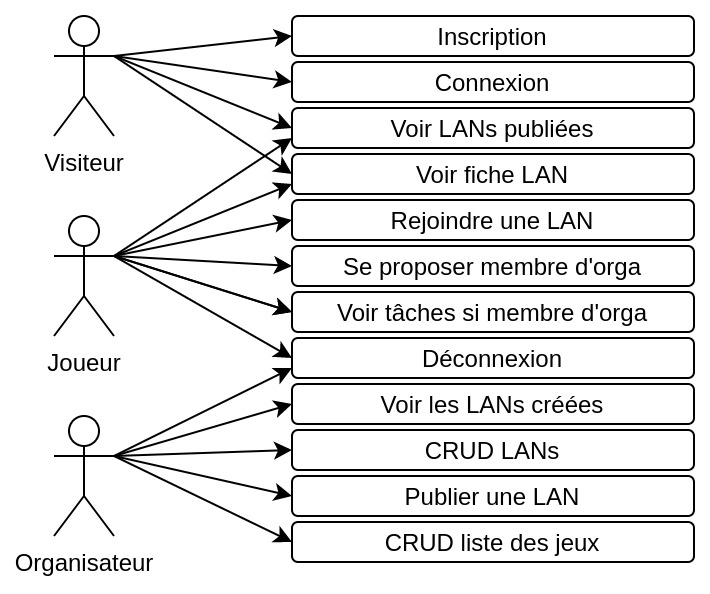
\includegraphics[scale=.40]{images/cas_utilisation.jpg}
\caption{Diagramme des cas d'utilisations}
\label{}
\end{figure}

\subsection{Diagramme de navigation}
\begin{figure}[H]
\centering
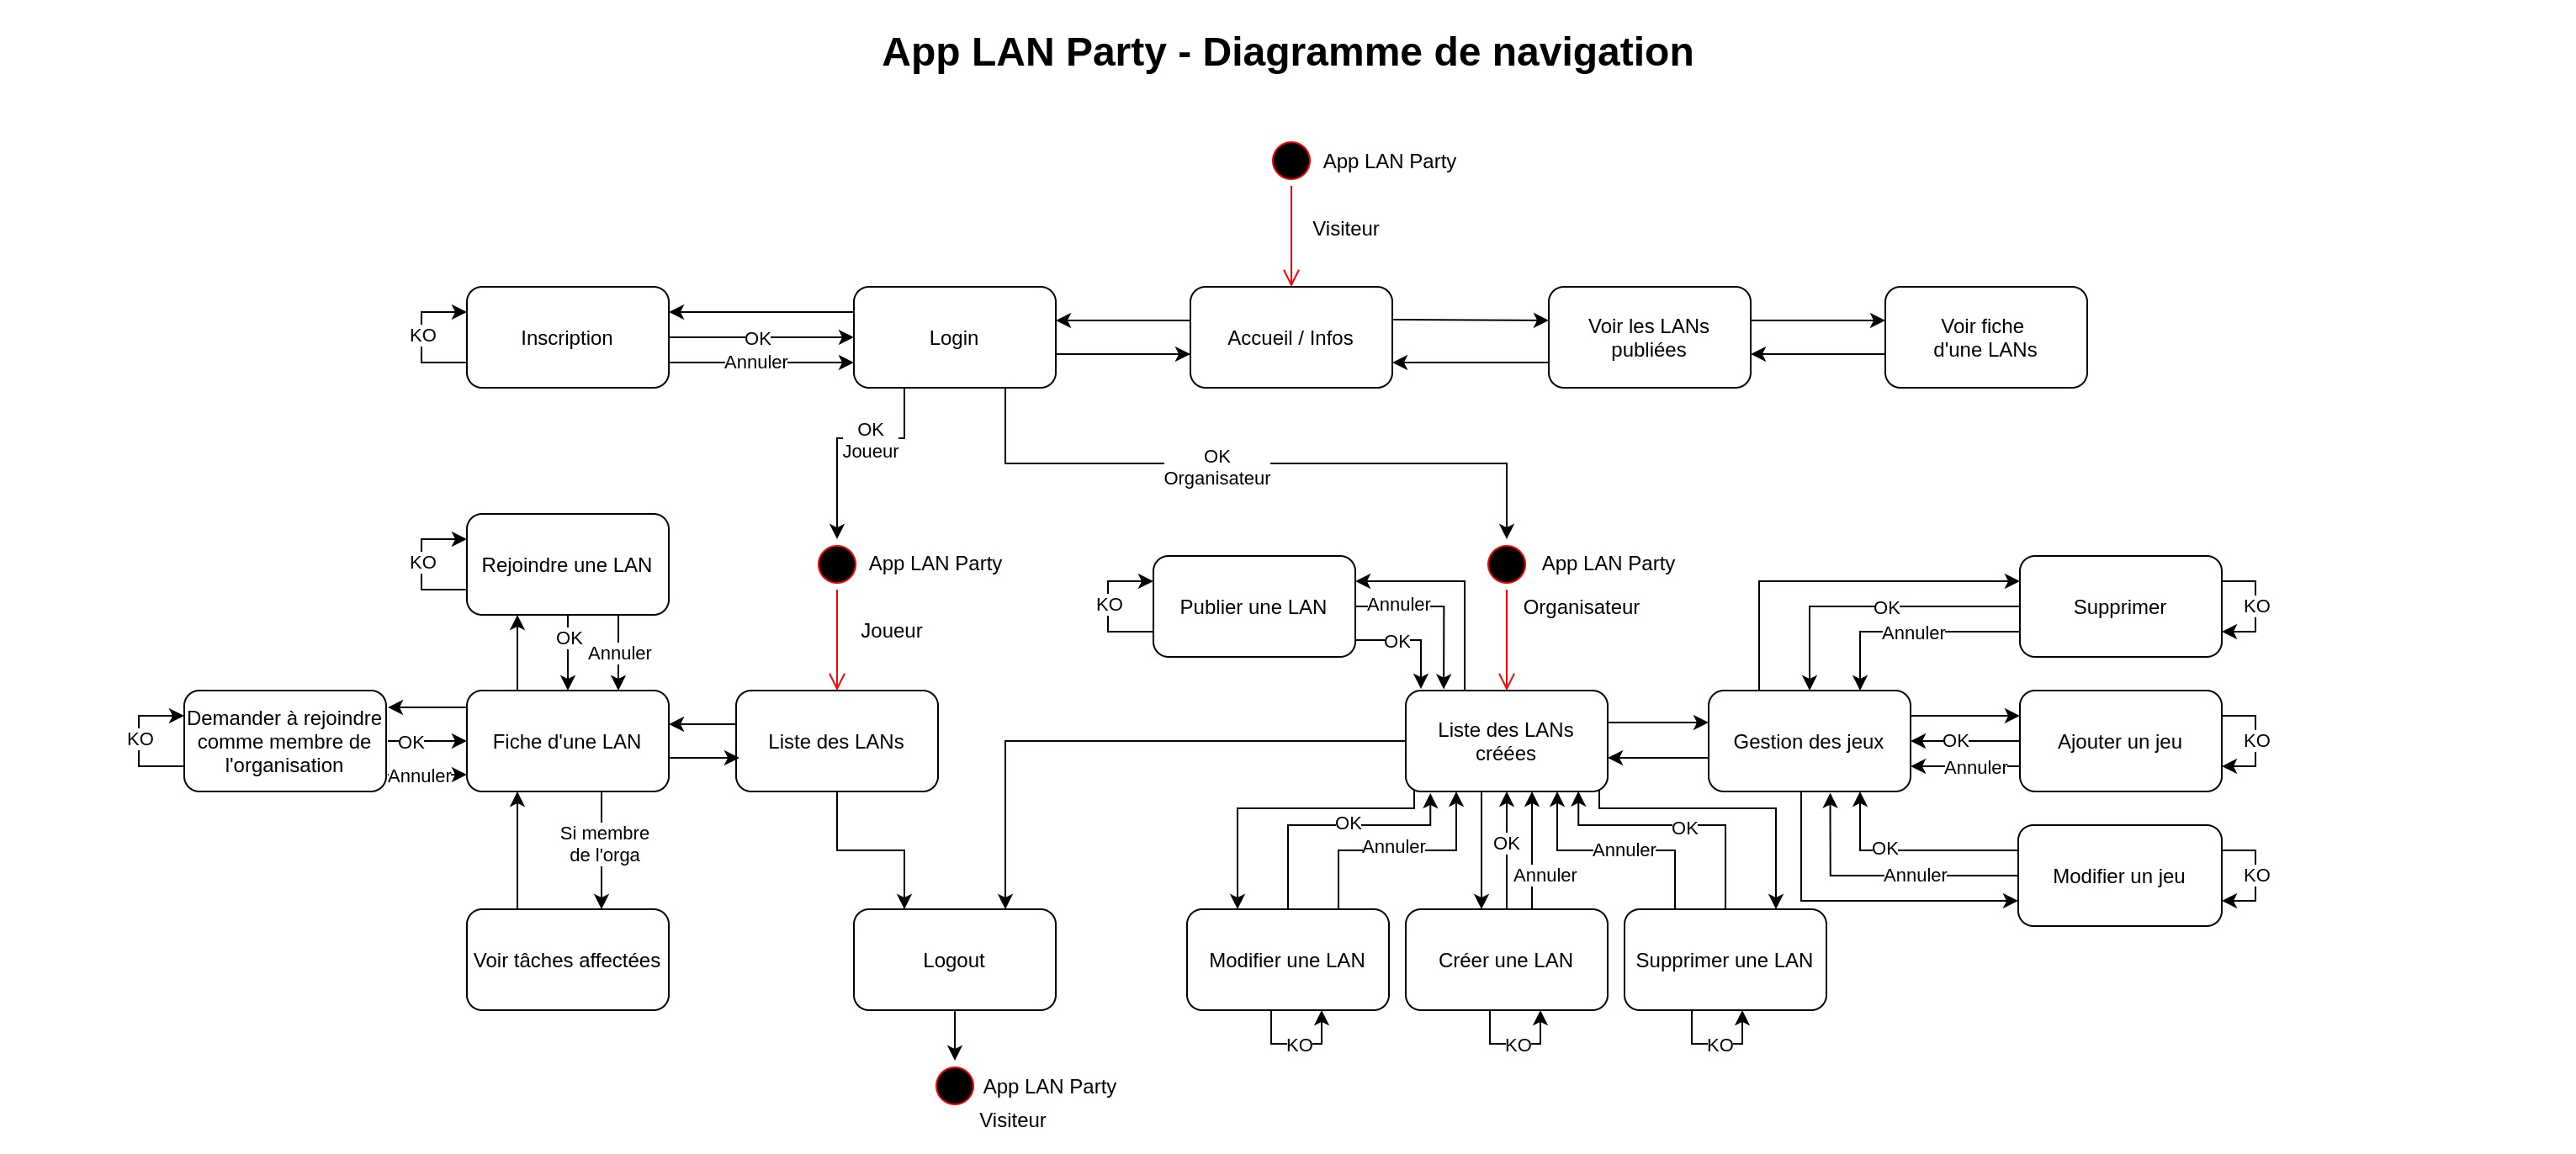
\includegraphics[scale=0.21,angle=90,origin=c]{images/navigation.jpg}
\caption{Diagramme de navigation}
\label{}
\end{figure}


Le site seras donc composer de trois parties, la partie commune aux trois utilisateur, la partie accessible par les joueur et celle uniquement accessible par les organisateur.
\newline

Dans la partie commune on retrouve donc la page d'accueil, le système d'inscription/connexion et la liste des LANs publiées dans lesquelles ont peut naviguer librement. 
\newline

Lorsque l'on se connecte en temps que joueur, on peut accéder à la liste des LANs mais avec la possibilité d'en rejoindre une. De plus si le joueur se propose comme membre d'organisation, il peut accéder aux tâches que les organisateur aurait pu leur donner. 
\newline

Finalement, un organisateur peut accéder à la liste des LANs publiées ou non, et faire toutes les actions possible sur elles.
\newpage
\subsection{Analyse de la base de données}

Notre base de données se compose de deux partie principales : la première contient tous se qui touche aux utilisateurs, le seconde tous se qui touche aux LANs. 
\newline

Les utilisateurs ont leurs propres table, mais possèdes aussi une tables permettant de modéliser les rôles (joueur ou organisateur), et une table correspondant aux tâches qui peut être attribué aux joueurs. 
\newline

Les LANs, en plus de leurs table propre, possèdent des tables pour les tournois, les jeux, le matériel et les salles. 
\newline

Les liens entre ses deux grandes partie sont le fait que les joueurs s'inscrivent aux LANs.
\newline

Voici le MCD que nous avons conçu à partir de ses informations : 

\begin{figure}[htp]
\centering
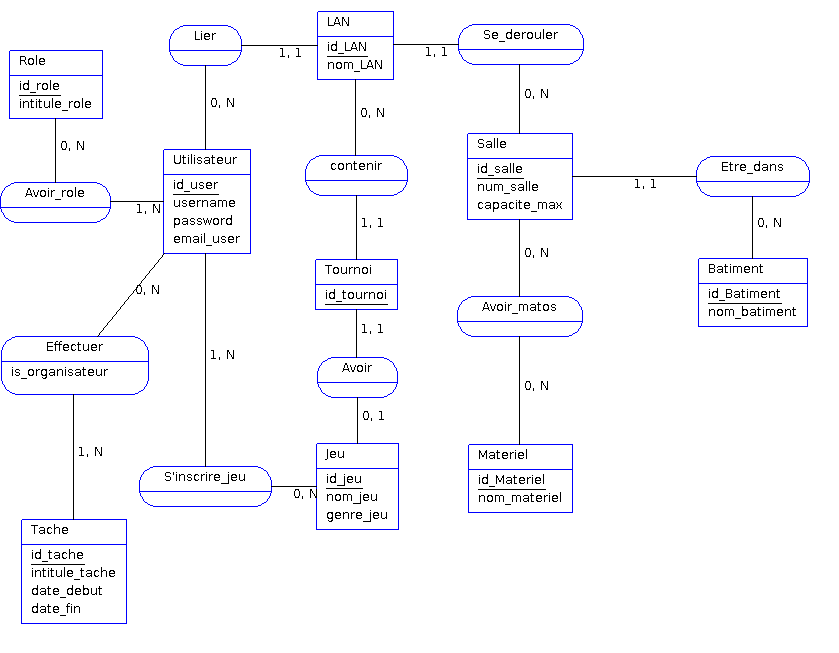
\includegraphics[scale=0.50]{images/mcd.png}
\caption{MCD de l'application}
\label{}
\end{figure}

\newpage

\section{Détoulement du développement}

\subsection{Organisation}

Bien évidemment, les circonstances actuelles ont eu une important impact sur l'organisation du travail. Nous avons donc organisé notre travail en conséquence car nous uniquement travaillé à distance sur le projet. Pour cela nous avons utilisés pour communiquer le programme Discord. Toutes les décisions ont été prise en ce consultant sur notre conversation. Nous avons privilégié la communication écrite car toutes les conditions n'étaient pas réuni pour organisé les conversations en vocale. Nous effectuions une mise au point tous les quelques jours et prévenons de nos avancements les autres membres. Pour le partage des sources nous avons utilisé Git et mis en ligne le repo sur GitHub.

\subsection{Partage du travail}

Nous avons tous d'abord avant de commencer le projet, chacun de notre côté, remis nos mains sur le framework
Laravel pour reprendre connaissances des différents concepts, leurs mises en place et les changements proposé par la sortie de la version 7 de Laravel.

Du à la petite taille de notre équipe, nous avons décider de partager le travail au fur et à mesure de notre progression. 

La première étape à donc été la phase de conception, décrite dans la première partie de ce rapport. 
\newpage

\section{Présentation de l'application}

\subsection{Partie publique}
Lorsque l'on se connecte à l'application, nous atterrissons sur la page d'accueil. Sur celle-ci nous retrouvons un liens permettant d'accéder à la liste des LANs, ainsi que les liens pour les formulaires de connexion et d'inscription.

\begin{figure}[H]
\centering
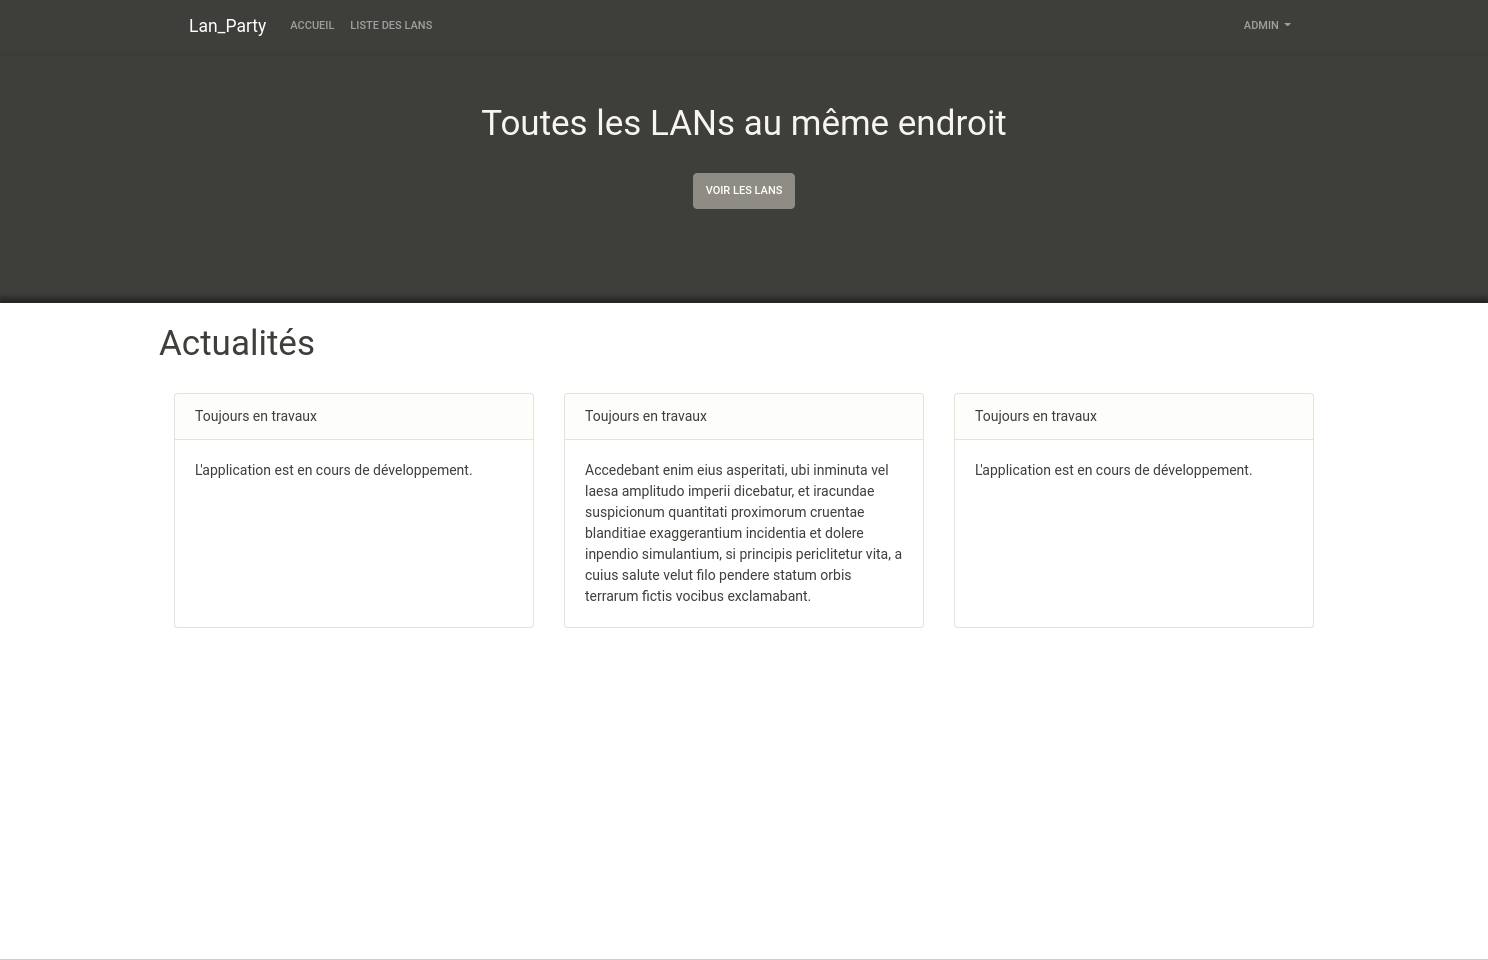
\includegraphics[scale=0.20]{images/accueil.png}
\caption{Page d'accueil}
\label{}
\end{figure}

\begin{figure}[H]
\centering
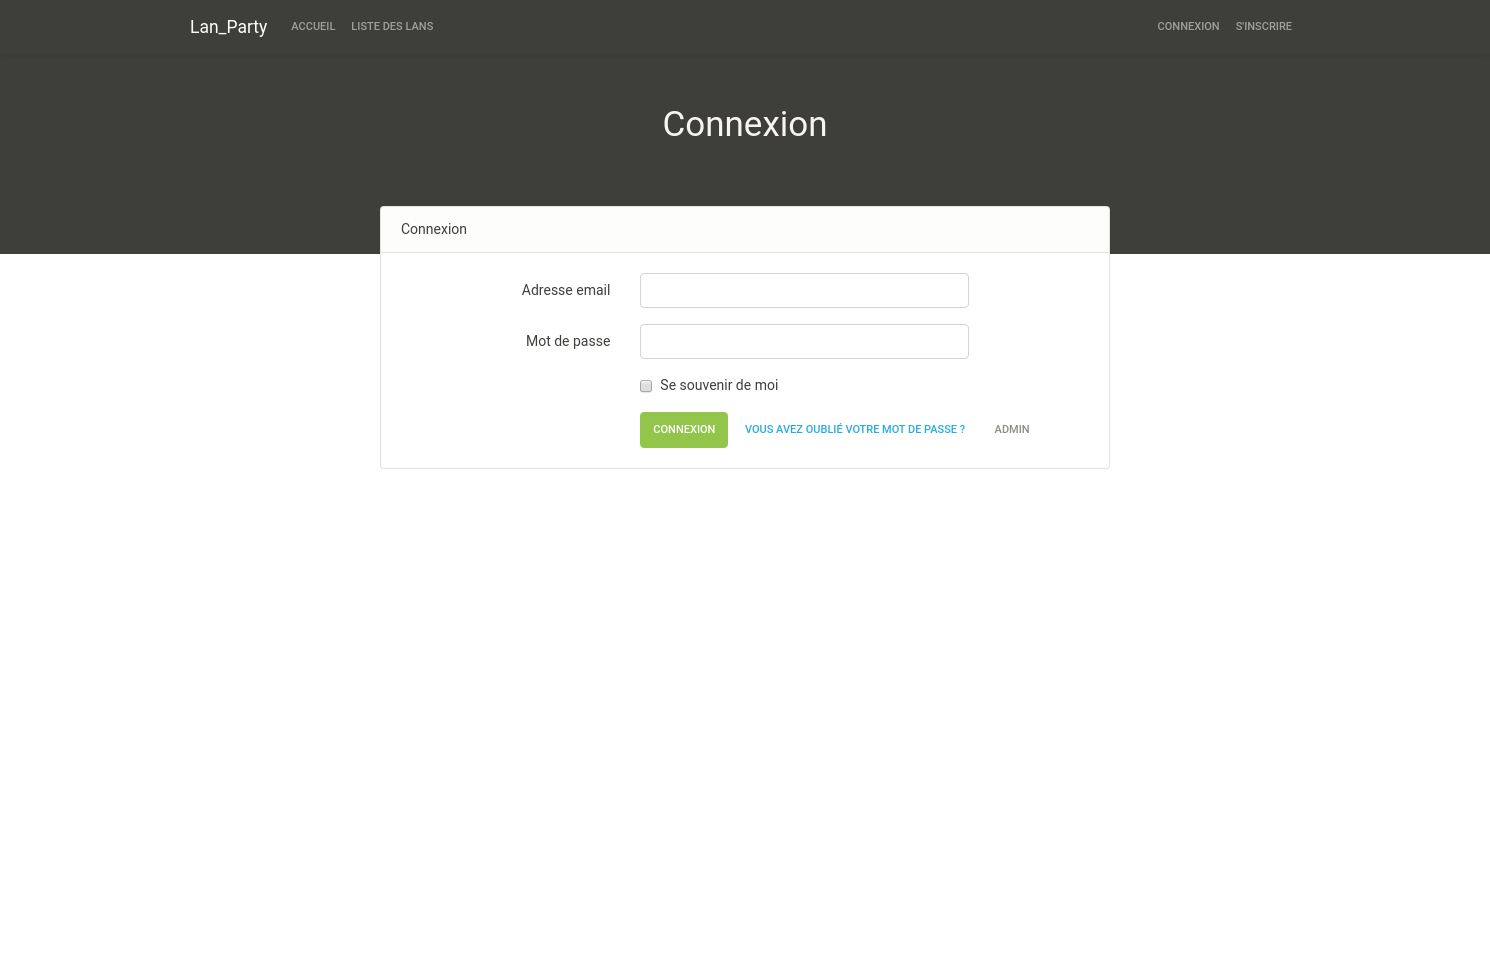
\includegraphics[scale=0.20]{images/connexion.jpg}
\caption{Page de connexion}
\label{}
\end{figure}

\begin{figure}[H]
\centering
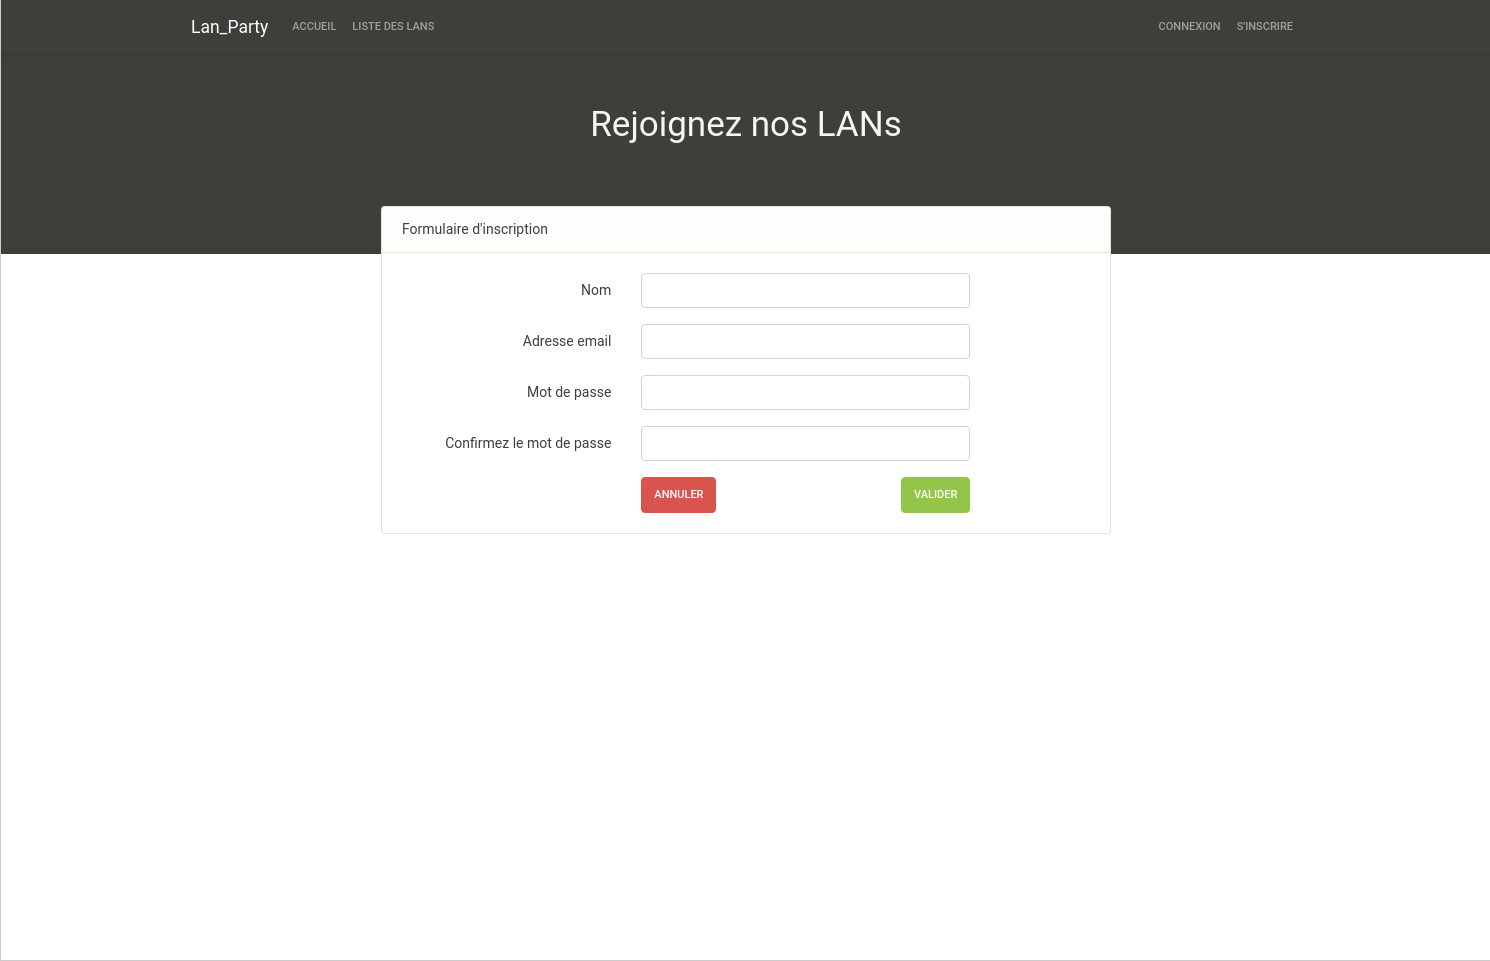
\includegraphics[scale=0.20]{images/inscription.png}
\caption{Page d'inscription}
\label{}
\end{figure}

\begin{figure}[H]
\centering
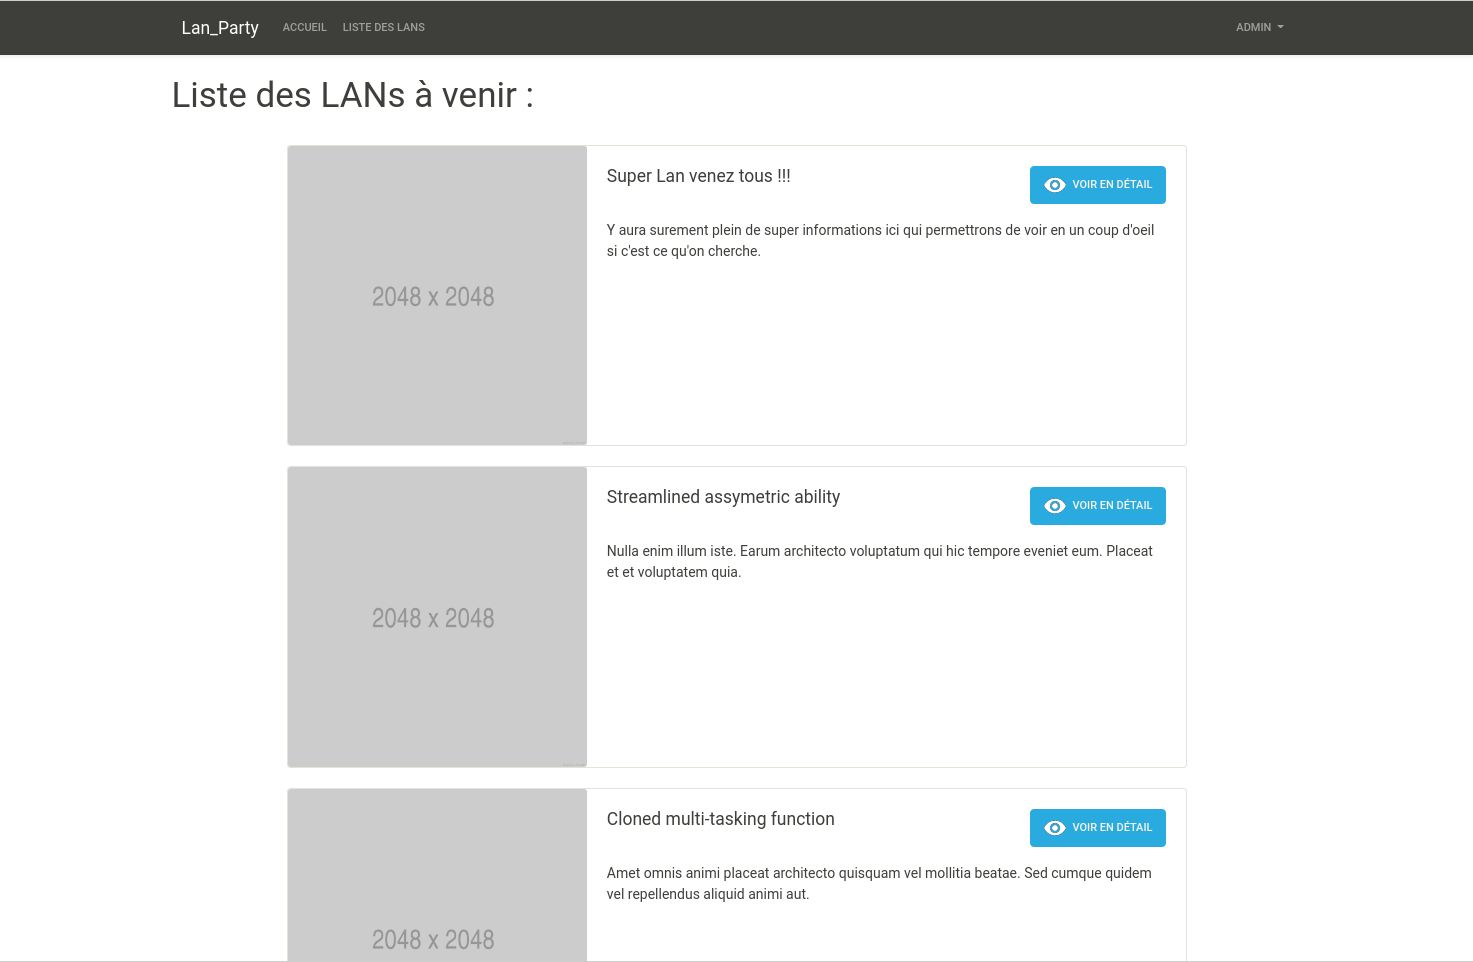
\includegraphics[scale=0.20]{images/liste.png}
\caption{Liste des Lans}
\label{}
\end{figure}

\subsection{Partie Joueur}

\subsection{Partie Organisateur}

\end{document}
